\chapter{Vectorized training of model ensembles}
\label{app:torchstrap}

The statistical uncertainties of the unbinned unfolding in Ch.~\ref{ch:angularities} are obtained by replacing every classifier of MultiFold with an ensemble of independently trained replicas (Sec.~\ref{sec:bootstrap}).
%
This is the bootstrap idea~\cite{Efron:1979bootstrap} applied to neural networks, where an ensemble of networks trained on resampled data also gives a well-calibrated estimate of the uncertainty of their prediction~\cite{Lakshminarayanan:2016ensembles}.
%
A MultiFold unfolding trains four classifiers per iteration, and it is repeated for every systematic variation, so an ensemble of \(N\) replicas multiplies an already long chain of trainings by \(N\).
%
This appendix describes \emph{torchstrap}\footnote{\url{https://github.com/TanmayPani/torchstrap}}, a PyTorch~\cite{Paszke:2019pytorch} library written for this thesis that trains all \(N\) replicas of an ensemble at once on a single GPU, as one vectorized computation rather than a loop over models.

\section{The cost of training replicas one by one}
\label{sec:tsMotivation}
The classifiers used here are small multi-layer perceptrons (MLPs), with a few hundred thousand parameters, trained on mini-batches of a few thousand jets.
%
Every operation of their training step, a matrix multiplication, an activation or an optimizer update, is a separate \emph{kernel} launched on the GPU, and a kernel acting on such small tensors finishes in a time comparable to the overhead of launching it.
%
Training \(N\) replicas one after the other, or in \(N\) separate processes, therefore multiplies the number of launches by \(N\) while leaving the GPU mostly idle, and separate processes in addition duplicate the memory of the framework itself.

The replicas, however, share their architecture and differ only in the values of their parameters and in the data they see.
%
For a dense layer with weights \(\Lambda^a_{\ b}\), acting on an input \(x_a\) as \(y_b = \Lambda^a_{\ b}\,x_a\), the \(N\) replicas
\begin{equation}
	y^{k}_{b} = \Lambda^{a,k}_{\ b}\,x^{k}_{a}, \qquad 1 \leq k \leq N,
	\label{eq:batchedLayer}
\end{equation}
are a single \emph{batched} matrix multiplication over the extra index \(k\), which runs as one kernel instead of \(N\).
%
Rewriting a whole model in this form by hand is error prone, but PyTorch provides the transformation \texttt{torch.func.vmap}, which turns a function written for one replica into one that acts on tensors with an additional leading replica dimension, adding the index \(k\) of Eq.~\ref{eq:batchedLayer} to every operation.
%
Fig.~\ref{fig:tsEnsembles} shows the three configurations discussed in this appendix: a single model, an ensemble of replicas trained on the same data, and a bootstrap ensemble in which every replica is trained on its own resample.

% ---------------------------------------------------------------------------
% Drawing helpers for this appendix
\tikzset{
	tsnode/.style={circle, draw=#1!60!black, fill=#1!25, thick, minimum size=4.2mm, inner sep=0pt},
	tsnode/.default=blue,
	tsedge/.style={draw=blue!30!black!40, line width=0.35pt},
	tscard/.style={draw=black!55, rounded corners=3pt, fill=white, line width=0.5pt},
	tscell/.style={draw=black!50, fill=#1, minimum width=9mm, minimum height=4.5mm, inner sep=0pt, font=\scriptsize},
	tscell/.default=blue!12,
	tsarrow/.style={-{Latex[length=2.2mm]}, thick, red!70!black},
}
% \tsMLP{x}{y}: a 2-4-4-1 MLP inside a card, lower-left corner of the card at (x,y)
\newcommand{\tsMLP}[2]{%
	\begin{scope}[shift={(#1,#2)}]
		\draw[tscard] (0,0) rectangle (3.3,2.0);
		\foreach \i in {1,2} \coordinate (in\i) at (0.35, {1.0+0.45*(\i-1.5)});
		\foreach \i in {1,...,4} \coordinate (ha\i) at (1.25, {1.0+0.42*(\i-2.5)});
		\foreach \i in {1,...,4} \coordinate (hb\i) at (2.15, {1.0+0.42*(\i-2.5)});
		\coordinate (out) at (2.95, 1.0);
		\foreach \i in {1,2} \foreach \j in {1,...,4} \draw[tsedge] (in\i) -- (ha\j);
		\foreach \i in {1,...,4} \foreach \j in {1,...,4} \draw[tsedge] (ha\i) -- (hb\j);
		\foreach \i in {1,...,4} \draw[tsedge] (hb\i) -- (out);
		\foreach \i in {1,2} \node[tsnode=green] at (in\i) {};
		\foreach \i in {1,...,4} \node[tsnode] at (ha\i) {};
		\foreach \i in {1,...,4} \node[tsnode] at (hb\i) {};
		\node[tsnode=red] at (out) {};
	\end{scope}}
% \tsCard{x}{y}: an empty card of the same size, for replicas behind the front one
\newcommand{\tsCard}[2]{\draw[tscard] (#1,#2) rectangle ++(3.3,2.0);}
% \tsData{x}{y}{label of sample i}{fill}: a 2 x 4 block of (x, y) inputs, lower-left corner at (x,y)
\newcommand{\tsData}[4]{%
	\begin{scope}[shift={(#1,#2)}]
		\foreach \c/\s in {0/0, 1/1, 3/S} {
			\node[tscell=#4, anchor=south west] at ({0.9*\c}, 0.45) {\(x_{#3{\s}}\)};
			\node[tscell=#4, anchor=south west] at ({0.9*\c}, 0) {\(y_{#3{\s}}\)};
		}
		\node[tscell=#4, anchor=south west] at (1.8, 0.45) {\(\cdots\)};
		\node[tscell=#4, anchor=south west] at (1.8, 0) {\(\cdots\)};
	\end{scope}}
\newcommand{\tsIdx}[1]{#1}
\newcommand{\tsBoot}[1]{r_k(#1)}
% ---------------------------------------------------------------------------

\begin{figure}[htbp]
	\centering
	\begin{tikzpicture}[font=\small]
		% (a) single model
		\node[anchor=west, font=\bfseries] at (-0.9, 1.0) {(a)};
		\tsData{0}{0.55}{\tsIdx}{blue!12}
		\tsMLP{4.3}{0}
		\draw[tsarrow] (3.65,1.0) -- (4.3,1.0);
		\node[font=\scriptsize] at (5.95,-0.25) {\(\theta\)};
		\node[anchor=west, align=left] at (8.6,1.0) {\(p(x, y;\,\theta)\)\\[1pt]\scriptsize one set of parameters \(\theta\)};

		% (b) ensemble, same data
		\begin{scope}[yshift=-3.3cm]
			\node[anchor=west, font=\bfseries] at (-0.9, 1.0) {(b)};
			\tsData{0}{0.55}{\tsIdx}{blue!12}
			\foreach \k in {4,3,2,1} \tsCard{4.3+0.16*\k}{0.16*\k}
			\tsMLP{4.3}{0}
			\draw[tsarrow] (3.65,1.0) -- (4.3,1.0);
			\node[font=\scriptsize] at (5.95,-0.25) {\(\theta^{(1)}\)};
			\node[font=\scriptsize, anchor=south west] at (8.24,2.3) {\(\theta^{(N)}\)};
			\node[anchor=west, align=left] at (8.6,1.0) {\(p(x, y;\,\theta^{(k)})\), \(k = 1\ldots N\)\\[1pt]\scriptsize same data, different initializations};
		\end{scope}

		% (c) bootstrap ensemble
		\begin{scope}[yshift=-6.9cm]
			\node[anchor=west, font=\bfseries] at (-0.9, 1.0) {(c)};
			\foreach \k in {4,3,2,1} {
				\fill[white] ({0.16*\k},{0.55+0.16*\k}) rectangle ++(3.6,0.9);
				\draw[black!40, rounded corners=1pt] ({0.16*\k},{0.55+0.16*\k}) rectangle ++(3.6,0.9);
			}
			\tsData{0}{0.55}{\tsBoot}{orange!15}
			\foreach \k in {4,3,2,1} \tsCard{4.3+0.16*\k}{0.16*\k}
			\tsMLP{4.3}{0}
			\draw[tsarrow] (3.65,1.0) -- (4.3,1.0);
			\node[font=\scriptsize] at (5.95,-0.25) {\(\theta^{(1)}\)};
			\node[font=\scriptsize, anchor=south west] at (8.24,2.3) {\(\theta^{(N)}\)};
			\node[anchor=west, align=left] at (8.6,1.0) {\(p(x, y;\,\theta^{(k)})\), \(k = 1\ldots N\)\\[1pt]\scriptsize replica \(k\) sees the resample \(r_k\)};
		\end{scope}
	\end{tikzpicture}
	\caption[Single model, ensemble and bootstrap ensemble of MLP classifiers]{Three ways of training an MLP classifier on a dataset of \(S\) two-dimensional points \((x_i, y_i)\). (a) A single model with parameters \(\theta\). (b) An ensemble of \(N\) replicas with independently initialized parameters \(\theta^{(k)}\), all trained on the same data. (c) A bootstrap ensemble, in which replica \(k\) is trained on its own resample of the data, the points \(r_k(i)\) drawn at random for that replica. In (b) and (c) the stack of replicas is evaluated and trained as one batched model.}
	\label{fig:tsEnsembles}
\end{figure}

\section{Stateless models and vectorized training}
\label{sec:tsStateless}
A PyTorch model object normally owns its parameters, which ties one set of parameters to one model.
%
torchstrap separates the two: the model is kept only as a description of the computation, on PyTorch's \texttt{meta} device where it holds no data, and the parameters and buffers of all replicas are kept outside of it, stacked along a leading dimension of size \(N\).
%
The forward pass of one replica is the model applied to one slice of these stacks through \texttt{torch.func.functional\_call}, and \texttt{vmap} over the slices evaluates all replicas in a single pass.
%
The gradients are obtained the same way, by vectorizing \texttt{torch.func.grad\_and\_value} of the per-replica loss, so a training step is written once for a single model and runs for the whole ensemble.
%
Random operations such as dropout are vectorized with independent random numbers for every replica, and the replicas are created with independent initial parameters.

The replica dimension is carried through every part of the training that differs between replicas:
\begin{itemize}
	\item \emph{Data.} The subsamples of Sec.~\ref{sec:bootstrap} are drawn for all replicas at once, as an \((N, n)\) tensor of indices in which row \(k\) is the random subsample and training/validation split of replica \(k\), or a with-replacement bootstrap resample. The mini-batches are consecutive column blocks of this tensor, which are views and require no copy, so every replica receives its own batch of jets in the same step.
	\item \emph{Hyperparameters.} The learning rate and the other optimizer settings are \((N,)\) vectors rather than numbers, so every replica can follow its own learning-rate schedule, and a scan of a hyperparameter can itself be run as an ensemble.
	\item \emph{Callbacks.} Early stopping, checkpointing and learning-rate scheduling act per replica. When the validation loss of replica \(k\) stops improving, early stopping sets the \(k\)-th entry of an \((N,)\) \emph{active mask} to false, and the replica is frozen while the others continue to train.
	\item \emph{Metrics.} Losses and scores, such as the accuracy and the area under the ROC curve, are computed for all replicas at once and returned as \((N,)\) vectors, together with the score of the ensemble-averaged prediction.
\end{itemize}

\section{Consolidated parameters and a fused optimizer}
\label{sec:tsOptimizer}
After the forward and backward passes, the optimizer updates every parameter tensor of every replica.
%
With the optimizers of PyTorch this is again a loop over replicas, and within each replica over its parameter tensors.
%
torchstrap instead stores all parameters of all replicas in one contiguous \emph{consolidated} buffer of shape \((N, T)\), where \(T\) is the number of parameters of one replica, shown in Fig.~\ref{fig:tsConsolidated}.
%
The weight and bias tensors of the model are views into this buffer, located through a table of their names, shapes and offsets, so the model sees ordinary tensors while the optimizer sees one matrix.
%
The gradients and the optimizer states, e.g.\ the first and second moments of Adam, share the same layout.
%
The width \(T\) is padded to a multiple of four elements, so that every row starts at an aligned address and the kernel can use vectorized memory access for the whole ensemble; the padding stays zero throughout the training.

\begin{figure}[htbp]
	\centering
	\begin{tikzpicture}[font=\small, x=0.86cm, y=1cm]
		% segments of one row: start / width / colour
		\def\rowh{0.55}
		\def\segs{0/1.4/blue!25, 1.4/0.35/blue!45, 1.75/3.2/green!25, 4.95/0.35/green!45, 5.3/3.2/orange!25, 8.5/0.35/orange!45, 8.85/0.8/red!20, 9.65/0.15/red!40, 9.8/0.2/black!10}
		\foreach \ytop/\lab/\mval/\mcol in {0/1/1/green!25, -0.55/2/0/red!25, -1.1/3/1/green!25, -2.0/N/1/green!25} {
			\foreach \x/\w/\c in \segs {
				\fill[\c] (\x,\ytop) rectangle ++(\w,-\rowh);
				\draw[black!60] (\x,\ytop) rectangle ++(\w,-\rowh);
			}
			\node[anchor=east] at (-0.1,\ytop-\rowh/2) {replica \lab};
			\node[draw, minimum size=4mm, inner sep=0pt, fill=\mcol, font=\scriptsize] at (11.3,\ytop-\rowh/2) {\mval};
		}
		% the frozen replica
		\fill[white, opacity=0.6] (0,-0.55) rectangle (10.0,-1.1);
		\fill[pattern=north east lines, pattern color=black!45] (0,-0.55) rectangle (10.0,-1.1);
		\node at (4.9,-1.75) {\(\vdots\)};
		\node at (11.3,-1.75) {\(\vdots\)};
		% column labels: weights in the lower row, biases and padding staggered above
		\foreach \x/\w/\lab in {0/1.4/W^{(1)}, 1.75/3.2/W^{(2)}, 5.3/3.2/W^{(3)}, 8.85/0.8/W^{(4)}} {
			\node[font=\scriptsize] at ({\x+\w/2},0.22) {\(\lab\)};
		}
		\foreach \x/\w/\lab in {1.4/0.35/b^{(1)}, 4.95/0.35/b^{(2)}, 8.5/0.35/b^{(3)}, 9.65/0.15/b^{(4)}} {
			\draw[black!50] ({\x+\w/2},0.02) -- ({\x+\w/2},0.45);
			\node[font=\scriptsize, anchor=south] at ({\x+\w/2},0.42) {\(\lab\)};
		}
		\draw[black!50] (9.9,0.02) -- (10.3,0.62);
		\node[font=\scriptsize, anchor=south west] at (10.1,0.6) {pad};
		\node[font=\scriptsize, align=center, anchor=south] at (11.3,0.05) {active\\mask};
		\draw[decorate, decoration={brace, amplitude=5pt}] (0,0.95) -- (10.0,0.95) node[midway, above=6pt] {one replica: all parameters, \(T\) elements};
		% frozen annotation
		\draw[-{Latex[length=2mm]}, thick, black!60] (11.7,-0.825) -- ++(0.5,0) node[right, align=left, font=\scriptsize] {frozen:\\skipped};
		% chunk grid
		\foreach \x in {2.5,5.0,7.5} \draw[dashed, thick, black!70] (\x,0.05) -- (\x,-2.65);
		\foreach \i/\x in {0/1.25,1/3.75,2/6.25,3/8.75} \node[font=\scriptsize] at (\x,-2.85) {\i};
		\draw[-{Latex[length=2mm]}, thick] (-2.1,0.0) -- (-2.1,-2.55) node[midway, left, font=\scriptsize, align=right] {\texttt{blockIdx.y}\\= replica};
		\draw[-{Latex[length=2mm]}, thick] (0,-3.15) -- (10.0,-3.15) node[midway, below, font=\scriptsize] {chunks along \(T\) (\texttt{blockIdx.x})};
	\end{tikzpicture}
	\caption[Consolidated parameter buffer of an ensemble and the launch grid of the fused optimizer]{The consolidated \((N, T)\) buffer holding the parameters of all \(N\) replicas of a four-layer MLP. Each row is one replica, with its weight matrices \(W^{(l)}\) and bias vectors \(b^{(l)}\) stored one after another and padded to a multiple of four elements. The gradients and the optimizer states share this layout. The fused optimizer covers the buffer with a two-dimensional grid of thread blocks, one grid row per replica and one column per chunk of the row (dashed lines). A replica frozen by early stopping (hatched, active mask 0) is skipped by all of its blocks.}
	\label{fig:tsConsolidated}
\end{figure}

With this layout the update of the whole ensemble is a single elementwise operation on a few \((N, T)\) matrices.
%
torchstrap implements it as fused kernels for the Adam optimizer~\cite{Kingma:2014adam}, including its variant with decoupled weight decay (AdamW~\cite{Loshchilov:2017adamw}) used in this thesis, and for SGD and Adagrad, with one C++ implementation for the CPU and one CUDA implementation for the GPU, registered as PyTorch operators.
%
A kernel reads each element of the parameters, gradients and moments once, updates it and writes it back, without allocating any temporary \((N, T)\) tensors, so it needs no more memory than a loop over replicas.
%
The GPU kernel is launched on the two-dimensional grid of Fig.~\ref{fig:tsConsolidated}, in which every block works on one chunk of one replica.
%
This makes the per-replica quantities cheap: the learning rate, the other hyperparameters and the step count used for the bias correction of Adam are read once per block from the \((N,)\) vectors, and a block whose replica is frozen returns immediately, so a frozen replica costs no memory traffic and its parameters remain exactly unchanged.
%
The arithmetic of the update is taken from the fused optimizers of PyTorch itself, and for every active replica the result is bit-for-bit identical to that of \texttt{torch.optim.Adam} with \texttt{fused=True}, which is enforced by the tests of the library.
%
The optimizer also composes with \texttt{vmap}, so the complete training step, forward pass, backward pass and parameter update, is written for one model and vectorized as a whole.

Tab.~\ref{tab:tsBenchmark} compares one Adam step of torchstrap with the straightforward alternative of \(N\) independent PyTorch optimizers stepped in a loop, for an MLP of the size used for the toy example below.
%
The speed-up is largest for small ensembles, where the launch overhead dominates, and settles at about a factor of three once the ensemble is large enough for the update to be limited by the memory bandwidth.
%
Late in a training, when early stopping has frozen most replicas, the skipped rows make the update another factor of four faster.

\begin{table}[htbp]
	\caption[Timing of one optimizer step for an ensemble]{Time of one Adam step for an ensemble of \(N\) MLP replicas with six parameter tensors and 265k parameters each, in single precision on an NVIDIA RTX 4070 Laptop GPU (median of 20 runs). The loop steps \(N\) independent \texttt{torch.optim.Adam} optimizers; torchstrap updates the consolidated buffer with one fused kernel. The peak memory is the same for both. The last row has 75\% of the replicas frozen.}
	\label{tab:tsBenchmark}
	\centering
	\begin{tabular}{r | r r | c}
		\hline
		\(N\) & Loop & torchstrap & Speed-up \Tstrut \Bstrut \\
		\hline
		8 & 796~\(\mu\)s & 140~\(\mu\)s & 5.7 \\
		32 & 3.22~ms & 1.18~ms & 2.7 \\
		100 & 9.38~ms & 3.23~ms & 2.9 \\
		100, 75\% frozen & -- & 0.80~ms & 4.0 (vs.\ all active) \\
		\hline
	\end{tabular}
\end{table}

\section{Toy example}
\label{sec:tsToy}
The effect of the three configurations of Fig.~\ref{fig:tsEnsembles} is illustrated with the two-spirals example of the torchstrap repository: a classifier separating two interleaved spirals of 100 points in total, smeared with Gaussian noise, a problem in which the decision boundary is only constrained where there are data.
%
An MLP with two hidden layers of 512 nodes is trained with Adam and a cosine learning-rate schedule, once as a single model and twice as an ensemble of 100 replicas trained in parallel, and the predicted probability of the classifier is shown in Fig.~\ref{fig:tsSpirals}.
%
The single model (left) draws a sharp boundary that separates the training points and extends arbitrarily into the regions without data.
%
An ensemble trained on the same data (middle) differs only through the initialization of its replicas, and its mean prediction is nearly identical to the single model, since all replicas learn the same points.
%
When every replica is trained on its own bootstrap resample (right), the replicas disagree where the data do not constrain the boundary, and the mean prediction is softened there, most visibly away from the spiral arms, while it stays confident where the points are dense.
%
This spread of the replicas is the quantity that Sec.~\ref{sec:bootstrap} uses as the statistical uncertainty of the unfolded distributions.

\begin{figure}[htbp]
	\centering
	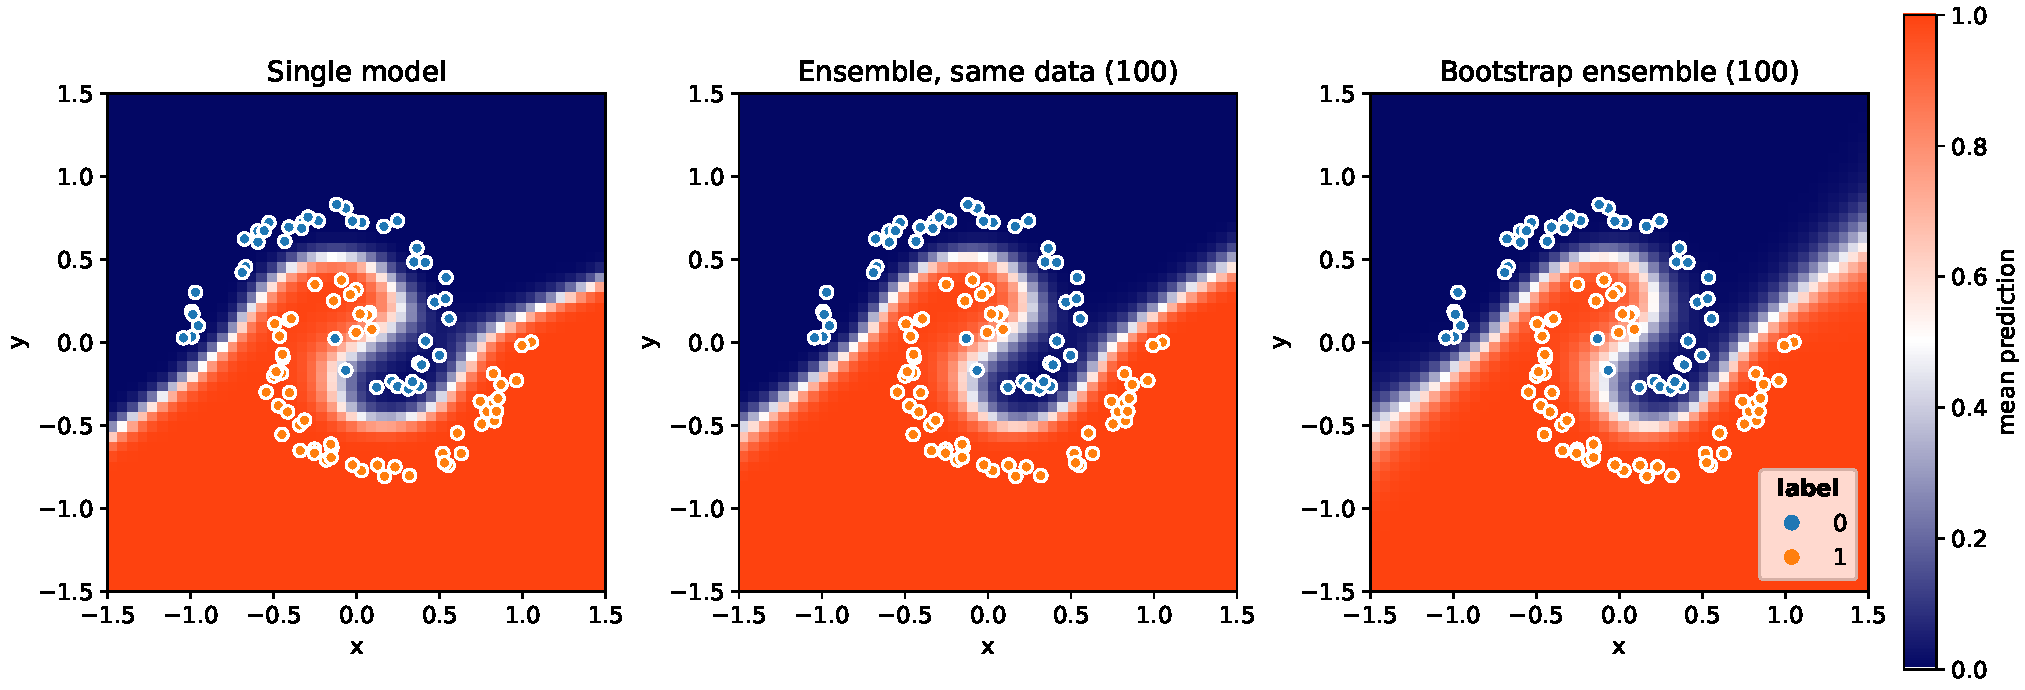
\includegraphics[width=\linewidth]{figures/torchstrap/spirals_predictions.pdf}
	\caption[Predictions of a single MLP and of MLP ensembles on the two-spirals problem]{Predicted probability of an MLP classifier trained on 100 points from two noisy spirals (blue: class 0, orange: class 1), for a single model (left), the mean of an ensemble of 100 replicas trained on the full dataset (middle), and the mean of a bootstrap ensemble of 100 replicas, each trained on its own resample (right). All replicas of an ensemble were trained simultaneously on one GPU.}
	\label{fig:tsSpirals}
\end{figure}

A bootstrap resample leaves out about 37\% of the points, which gives every replica a held-out \emph{out-of-bag} sample without a separate validation split.
%
The bootstrap ensemble uses it to monitor its training: the out-of-bag loss of every replica is computed in the same vectorized pass as the predictions and drives the per-replica learning-rate schedule, checkpointing and early stopping.
%
Fig.~\ref{fig:tsTraining} shows the resulting training history.
%
The training and out-of-bag losses of the replicas fall together for the first five epochs, after which the training loss keeps decreasing while the out-of-bag loss levels off at about 0.1, the onset of overfitting that the checkpoints of the best epoch guard against.
%
The out-of-bag loss of the individual replicas (right) differs by up to a factor of a few, reflecting the different points each replica was trained on, and the loss of the ensemble-averaged prediction lies below the mean loss of the replicas.

\begin{figure}[htbp]
	\centering
	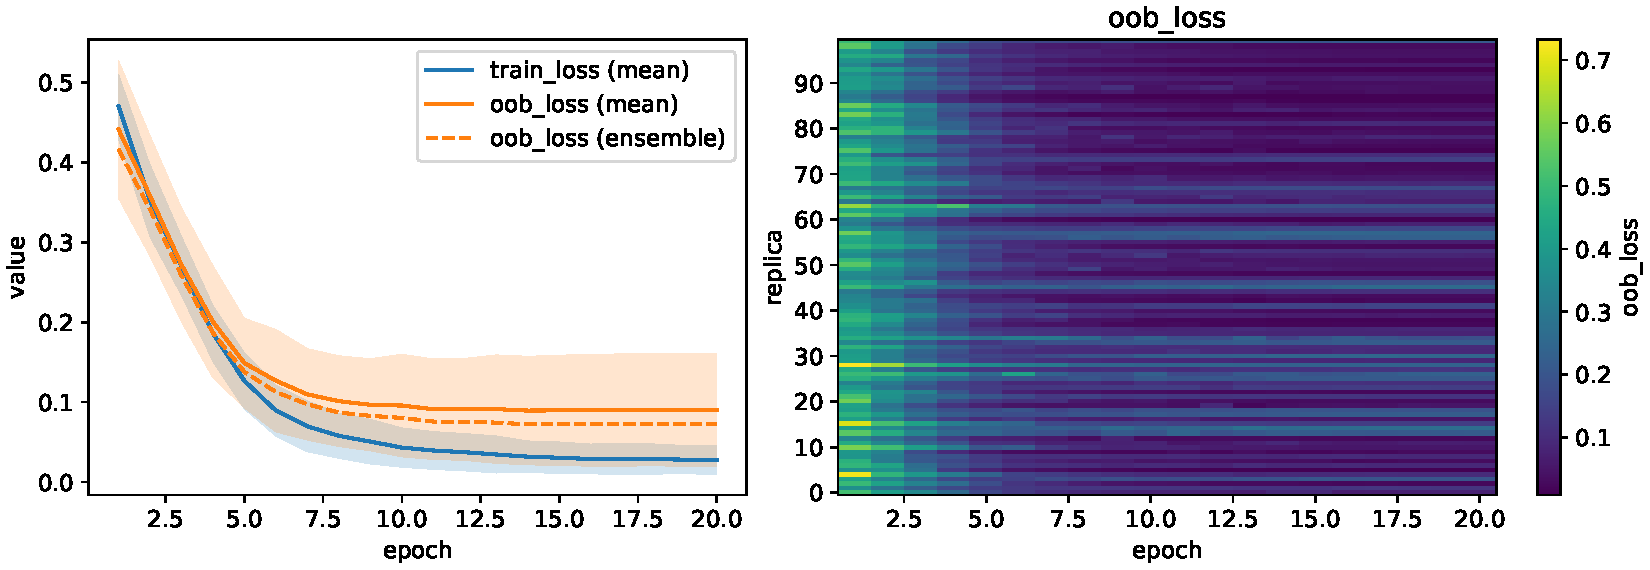
\includegraphics[width=\linewidth]{figures/torchstrap/spirals_training.pdf}
	\caption[Training history of the bootstrap ensemble of the two-spirals example]{Training history of the bootstrap ensemble of Fig.~\ref{fig:tsSpirals}. (Left) Training loss (blue) and out-of-bag loss (orange) averaged over the 100 replicas, with bands showing their spread, and the out-of-bag loss of the ensemble-averaged prediction (dashed). (Right) Out-of-bag loss of every replica (rows) in every epoch (columns).}
	\label{fig:tsTraining}
\end{figure}

\section{Use in this thesis}
\label{sec:tsUse}
In the MultiFold unfolding of the \pp measurement (Sec.~\ref{sec:ppUnfolding}), each of the four classifiers of an iteration is a torchstrap ensemble, and the replica index is carried through all classifiers and iterations, so that replica \(k\) is a complete unfolding of its own (Eq.~\ref{eq:replicaWeight}).
%
The per-replica subsamples of measured and simulated jets, the per-replica early stopping on the validation loss and the per-replica training histories of Fig.~\ref{fig:unfoldigLossAccAUC} are all provided by the mechanisms described above.
%
Because a frozen replica neither changes nor costs anything, the ensemble can be trained until its slowest replica has converged without degrading those that stopped earlier.
%
The whole ensemble, and with it the full set of systematic variations of Sec.~\ref{sec:ppSystematics}, were trained on a single laptop GPU, an NVIDIA RTX 4070 Laptop GPU with 8~GB of memory.
